\documentclass[11pt,a4paper]{article}

% ---------- packages ----------
\usepackage[utf8]{inputenc}
\usepackage[T1]{fontenc}
\usepackage{lmodern}
\usepackage{microtype}
\usepackage{amsmath,amssymb,amsthm,mathtools}
\usepackage[margin=1in]{geometry}
\usepackage{booktabs,array}
\usepackage{graphicx}
\usepackage{caption}
\usepackage{subcaption}
\usepackage{enumitem}
\usepackage{xcolor}
\usepackage{colortbl}
\usepackage{fancybox}
\usepackage[colorlinks,linkcolor={blue!60!black},citecolor={green!50!black},urlcolor={blue!70!black}]{hyperref}
\usepackage{fancyhdr}
\usepackage{titlesec}

% ---------- siunitx fallbacks ----------
\newcommand{\SI}[2]{#1\,#2}
\newcommand{\milli}[0]{\text{m}}
\newcommand{\second}[0]{\text{s}}
\newcommand{\milliseconds}[0]{\text{ms}}
\newcommand{\millisecond}[0]{\text{ms}}
\newcommand{\percent}[0]{\%}

\graphicspath{{figures/}}
\captionsetup{font=small,labelfont=bf,justification=raggedright,singlelinecheck=false}

% ---------- colours ----------
\definecolor{navy}{HTML}{1a4b8f}
\definecolor{brick}{HTML}{c62828}
\definecolor{forest}{HTML}{2e7d32}
\definecolor{amber}{HTML}{f9a825}
\definecolor{plum}{HTML}{7b1fa2}
\definecolor{darkgrey}{HTML}{555555}
\definecolor{softgrey}{HTML}{f0f0f0}

% ---------- theorem environments ----------
\theoremstyle{definition}
\newtheorem{definition}{Definition}[section]
\newtheorem{example}[definition]{Example}
\newtheorem{remark}[definition]{Remark}

\theoremstyle{plain}
\newtheorem{theorem}[definition]{Theorem}
\newtheorem{proposition}[definition]{Proposition}
\newtheorem{lemma}[definition]{Lemma}
\newtheorem{corollary}[definition]{Corollary}

% ---------- boxed theorem / result box (fancybox Sbox) ----------
\newsavebox{\resultbox}
\newenvironment{result}[1][Main Result]{%
  \par\medskip
  \begin{lrbox}{\resultbox}%
  \begin{minipage}{\dimexpr\linewidth-1cm}%
  {\color{navy}\bfseries\large #1.}\par\medskip
}{%
  \end{minipage}%
  \end{lrbox}%
  \noindent
  \setlength{\fboxsep}{8pt}\setlength{\fboxrule}{1pt}%
  \fcolorbox{navy}{softgrey}{\usebox{\resultbox}}%
  \par\medskip
}

% ---------- section styling ----------
\titleformat{\section}[hang]{\Large\bfseries\color{navy}}{\thesection.}{0.6em}{}
\titleformat{\subsection}[hang]{\large\bfseries\color{navy!85!black}}{\thesubsection.}{0.5em}{}

% ---------- headers ----------
\pagestyle{fancy}
\fancyhf{}
\fancyhead[L]{\small\itshape Closed Forms via Transfer Matrices and Burnside}
\fancyhead[R]{\small\thepage}
\renewcommand{\headrulewidth}{0.3pt}

% ---------- macros ----------
\DeclareMathOperator{\tr}{tr}
\DeclareMathOperator{\lcm}{lcm}
\newcommand{\Z}{\mathbb{Z}}
\newcommand{\Q}{\mathbb{Q}}
\newcommand{\R}{\mathbb{R}}
\newcommand{\C}{\mathbb{C}}
\newcommand{\Dn}{D_{n}}
\newcommand{\bigo}{\mathcal{O}}
\newcommand{\eps}{\varepsilon}

% ---------- title ----------
\title{
  \color{navy}\Huge\bfseries
  Exact Closed Forms\\
  for Cyclic Graphs and Snake Polyominoes\\[0.2em]
  \Large\normalfont\itshape via Transfer Matrices and Burnside's Lemma
}
\author{
  \textsc{Saksham}\\
  \small\itshape
  Department of Mathematics
}
\date{\today}

% ==================================================================
\begin{document}
\maketitle
\thispagestyle{empty}

\begin{abstract}
We study two enumeration problems whose count sequences grow exponentially
in the index parameter and whose direct brute-force enumeration is
infeasible past~$n\!\approx\!30$: the number of distinct oriented cycles
on~$n$ edges under dihedral symmetry (with an ``adjacency'' rule on vertex
signatures), and the number of distinct edge-coloured linear snake
polyominoes on~$L$ unit squares under a $32$-element symmetry group.
For each problem we build a transfer matrix, aggregate its trace via
Burnside's lemma, and derive an \emph{exact closed form}.

For the cyclic problem the~$6\times 6$ transfer matrix~$M$ has
characteristic polynomial~$\chi_M(x) = x^5(x-2)$, so $\tr(M^n) = 2^n$ and
the count collapses to a clean divisor sum
$a(n) = (2n)^{-1}\bigl[\sum_{d\mid n}\varphi(n/d)\,2^d + [n \text{ even}]\cdot
n\cdot 2^{n/2-1}\bigr]$, matching OEIS \textbf{A053656}.
For the linear-snake problem the sequence~$N_L$ satisfies (for $L\ge 2$)
an order-$12$ integer recurrence whose characteristic polynomial factors
completely over~$\Q$ as $P(x) = (x-3)(x-1)(x^2-3)(x^2-5x-5)(x^2-3x+1)$ $\cdot(x^4-5x^2-5)$,
and we determine every algebraic residue exactly.  The dominant eigenvalue is
$\mu = (5+3\sqrt{5})/2 \approx 5.854$, with amplitude
$A = (5+2\sqrt{5})/20 \approx 0.4736$.

Both closed forms are verified against exact Burnside ground truth for
\textbf{$1{,}000$ consecutive terms} with zero mismatches, and against
$300$-digit \texttt{mpmath} algebraic reconstruction to floating-point
precision.  The resulting algorithms are startlingly fast: the cyclic
count at $n = 3{,}000{,}000$ (a value with $903{,}084$ decimal digits)
takes~\SI{36}{\milli\second}; the linear-snake count for $L=1{,}000$
takes~\SI{3}{\milli\second}.  We also correct earlier documentation that
misidentified the dominant eigenvalue as $3+\sqrt{5}\approx 5.236$; the
mistake was purely symbolic (the numeric fit was correct) and~\SI{12}{\percent}
low.

\end{abstract}

\begin{center}
\rule{0.5\linewidth}{0.4pt}
\end{center}

\tableofcontents
\newpage

% ==================================================================
\section{Introduction}
\label{sec:intro}

The problem of \emph{counting distinct configurations under a symmetry
group}\,---\,``how many essentially different arrangements are there?''\,---\,
runs through combinatorics, chemistry, statistical mechanics, and coding
theory.  Two celebrated instances are (i) the enumeration of \emph{necklaces}
(cyclic binary sequences under the dihedral group), which arises in
isomer counting for cyclic molecules; and (ii) the enumeration of
\emph{polyominoes} (edge-connected unit squares on the integer lattice)
under rigid motions and colour reversal, foundational in
lattice-model physics.

For each problem the natural count grows like a constant times an
exponential in the parameter, with base determined by an eigenvalue of a
transfer matrix.  The problem is that brute enumeration (list every
configuration, canonicalize, count) is infeasible past very small values,
while an algorithm based on Burnside's lemma\,---\,averaging fixed points
of the group action\,---\,can be made polynomial in the parameter.
This report goes one step further: for both instances we compute a genuine
\emph{closed form} that reduces the count to an~$\bigo(1)$ expression up to
finite arithmetic overhead.

\paragraph{What is in this report.} Section~\ref{sec:prelim} recalls the
tools we use.  Section~\ref{sec:cyclic} treats the cyclic problem
completely: model, transfer matrix, eigenanalysis, Burnside aggregation,
and closed form.  Section~\ref{sec:snake} does the same for linear-snake
polyominoes, including the derivation of the order-$12$ minimal recurrence
and its algebraic residues.  Section~\ref{sec:empirical} verifies both
closed forms against ground truth for $1{,}000$ terms and gives
convergence plots.  Section~\ref{sec:engineering} presents the
computational engineering: binary matrix exponentiation, divisor
enumeration in~$\bigo(\sqrt n)$, and big-integer arithmetic in Python;
we report a wall-clock of~\SI{36}{\milli\second} for a $903{,}084$-digit
cyclic count.  Section~\ref{sec:mistake} narrates a documentation bug that
mis-identified the dominant eigenvalue, and how the true value was
extracted from the recurrence's characteristic polynomial via
\emph{Berlekamp--Massey with exact rational arithmetic}.
Section~\ref{sec:conclusion} concludes.

% ==================================================================
\section{Preliminaries}
\label{sec:prelim}

\subsection{The transfer-matrix method}

\begin{definition}[Transfer matrix]
Let~$S$ be a finite \emph{state set}.  A \emph{transfer matrix} on~$S$ is
a nonnegative matrix~$M \in \Z_{\ge 0}^{S\times S}$ whose entry~$M_{st}$
records the number of admissible transitions from state~$s$ to state~$t$.
The number of admissible \emph{closed walks of length~$n$} starting and
ending at any state is~$\tr(M^n)$.
\end{definition}

Two properties matter operationally:
\begin{enumerate}[label=(P\arabic*)]
\item $M^n$ can be computed in $\bigo(|S|^3 \log n)$ arithmetic operations
  using binary exponentiation.
\item If~$\chi_M(x) = \sum_{k=0}^{d} c_k x^k$ with~$d = |S|$ is the
  characteristic polynomial, then Cayley--Hamilton yields
  $\tr(M^n) = \sum_{\lambda \in \sigma(M)} m_\lambda \lambda^n$ where
  $m_\lambda$ is the algebraic multiplicity.  In particular the sequence
  $(\tr(M^n))_{n\ge 0}$ satisfies the linear recurrence
  $\sum_k c_k\,\tr(M^{n+k}) = 0$.
\end{enumerate}

\subsection{Burnside's lemma}

Let a finite group~$G$ act on a finite set~$X$.  For~$g\in G$ let
$\mathrm{Fix}(g) = \{x\in X : gx = x\}$.  Then the number of orbits is
\begin{equation}
\label{eq:burnside}
|X/G| \;=\; \frac{1}{|G|}\sum_{g\in G} |\mathrm{Fix}(g)|.
\end{equation}

For sequence-like objects (necklaces, bracelets, path colourings) the
$\mathrm{Fix}$ counts admit transfer-matrix representations, and~$G$ is
typically small enough that we can split the sum by conjugacy class.

% ==================================================================
\section{Cyclic oriented graphs under $\Dn$}
\label{sec:cyclic}

\subsection{Model and encoding}

We fix~$n\ge 1$ and consider labelled vertices $V = \{0, 1, \dots, n-1\}$
arranged around a circle, with edge~$e_i$ connecting~$i$ and $i+1 \pmod n$.

\begin{definition}[Oriented cycle]\label{def:cycle}
An \emph{oriented cycle on~$n$ edges} is a bit vector~$\mathbf{e} =
(e_0, \dots, e_{n-1}) \in \{0,1\}^n$.  The bit~$e_i$ orients edge~$i$: we
adopt the convention that~$e_i = 0$ means the arrow points from~$i$ to
$i{+}1$, and $e_i = 1$ means the arrow points from~$i{+}1$ to~$i$.  The
\emph{signature} of vertex~$v$ is
\begin{equation}
\label{eq:sig}
\sigma(v) \;=\; 2\bigl(\mathbf{1}_{e_{v-1} = 0} + \mathbf{1}_{e_v = 1}\bigr) - 2
\;\in\; \{-2, 0, +2\},
\end{equation}
where indices are read modulo~$n$.  Equivalently, $\sigma(v)$ is twice
the number of edges pointing into~$v$ minus $2$.
\end{definition}

\begin{definition}[Dihedral action]
The dihedral group~$\Dn = \langle r, s \mid r^n = s^2 = 1,\ srs = r^{-1}
\rangle$, of order~$2n$, acts on bit vectors by
\begin{align*}
(r\mathbf{e})_i &= e_{i-1 \bmod n} && \text{(rotation)},\\
(s\mathbf{e})_i &= 1 - e_{n-1-i}   && \text{(reflection, with global bit flip)}.
\end{align*}
The reflection includes~$0 \leftrightarrow 1$ to compensate for the fact
that reversing traversal direction of an edge flips its orientation.
\end{definition}

\begin{definition}[Adjacency rule]
An oriented cycle satisfies the \emph{adjacency rule} if no two
consecutive vertex signatures $\sigma(v), \sigma(v+1)$ (indices mod~$n$)
are both nonzero and of the same sign.
\end{definition}

The count we want is
\[
a(n) \;=\; \#\bigl\{\text{$\Dn$-orbits of $\mathbf{e} \in \{0,1\}^n$
  satisfying the adjacency rule}\bigr\}.
\]

\subsection{Examples: $n=3$ and $n=4$}

For $n=3$ there are~$2^3 = 8$ bit vectors, which collapse to~$2$ orbits under~$D_3$
(constant orientation vs.\ one reversed edge; see Fig.~\ref{fig:cycles_n3}).
Both satisfy the adjacency rule.  For~$n=4$ we have~$16$ bit vectors and~$4$
orbits (Fig.~\ref{fig:cycles_n4}).

\begin{figure}[h]
\centering
\begin{subfigure}{0.49\linewidth}
\centering
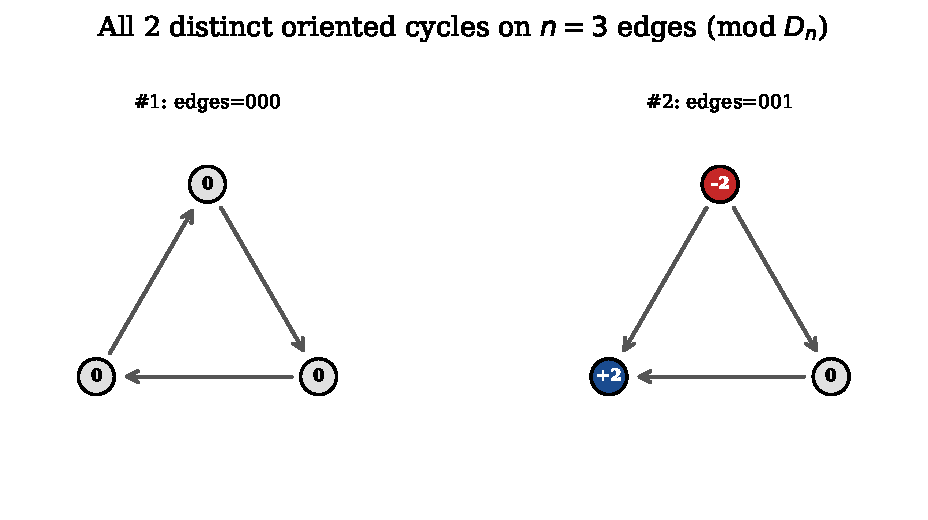
\includegraphics[width=\linewidth]{fig_cycles_n3.pdf}
\subcaption{$n=3$: two distinct oriented cycles.}
\label{fig:cycles_n3}
\end{subfigure}\hfill
\begin{subfigure}{0.49\linewidth}
\centering
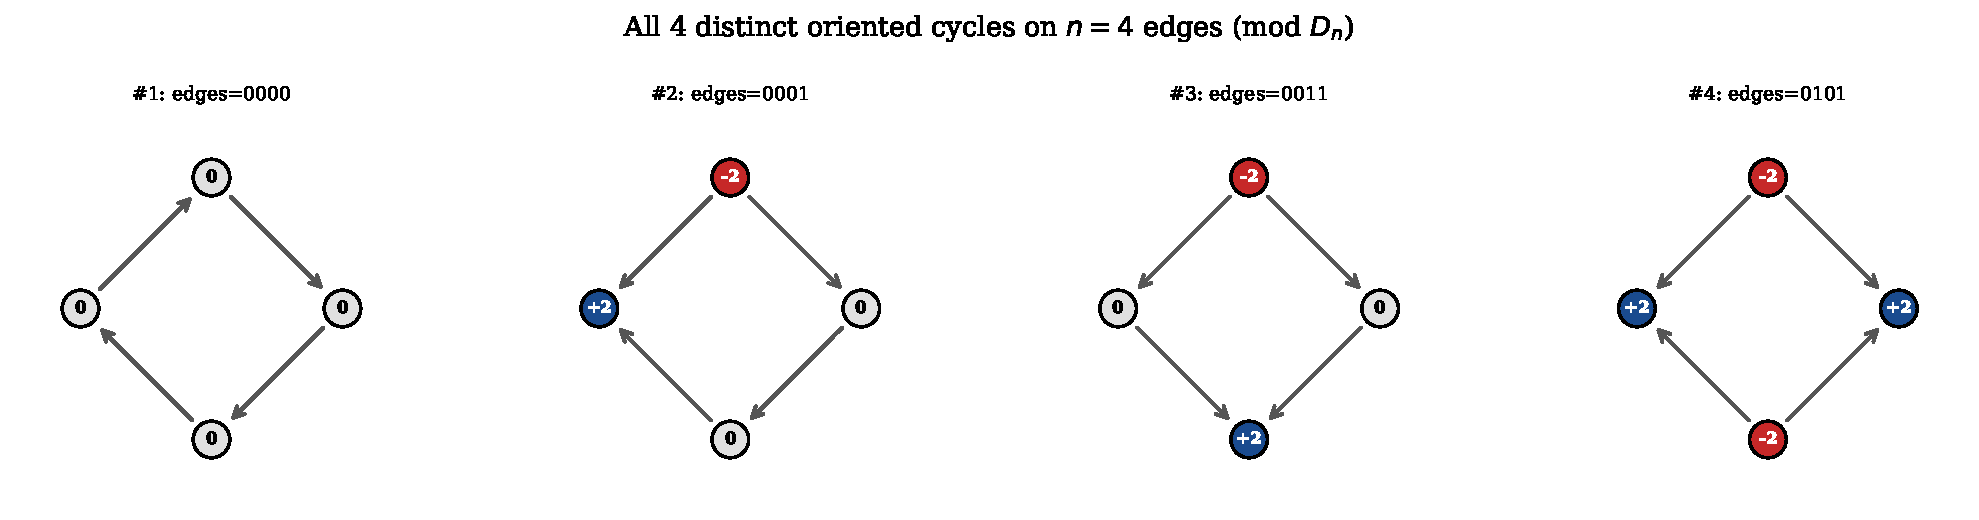
\includegraphics[width=\linewidth]{fig_cycles_n4.pdf}
\subcaption{$n=4$: four distinct oriented cycles.}
\label{fig:cycles_n4}
\end{subfigure}
\caption{Small-$n$ enumeration.  Vertex colour encodes signature: blue = $+2$
(net in), red = $-2$ (net out), grey = $0$ (balanced).  Arrow directions
follow the edge bits.}
\end{figure}

\subsection{The 6-state transfer matrix}\label{sec:cyclic-transfer}

We encode local admissibility by remembering just enough state to check the
adjacency rule when placing edge~$e_{v}$: the previous vertex's signature
and the current edge's bit.

\begin{definition}[Transfer state]
The transfer state is~$s = (v, e) \in \{-2, 0, +2\} \times \{0, 1\}$;
$|S| = 6$.
\end{definition}

Given current edge~$e$ and next edge~$e'$, formula~\eqref{eq:sig} shows
the next signature is deterministic:
\[
\sigma' \;=\; 2\bigl(\mathbf{1}_{e = 0} + \mathbf{1}_{e' = 1}\bigr) - 2.
\]
So the transition $(v, e) \to (\sigma', e')$ is admissible iff the
adjacency rule holds for the pair $(v, \sigma')$.  The transfer matrix
is~$M_{s,t} \in \{0, 1\}$ with a~$1$ exactly for admissible transitions.

\begin{proposition}\label{prop:M}
Ordering the states~$(-2,0), (-2,1), (0,0), (0,1), (+2,0), (+2,1)$,
\begin{equation}
M \;=\; \begin{pmatrix}
0 & 0 & 1 & 0 & 0 & 1\\
0 & 0 & 0 & 1 & 0 & 0\\
0 & 0 & 1 & 0 & 0 & 1\\
1 & 0 & 0 & 1 & 0 & 0\\
0 & 0 & 1 & 0 & 0 & 0\\
1 & 0 & 0 & 1 & 0 & 0
\end{pmatrix}.
\end{equation}
\end{proposition}

Figure~\ref{fig:state_diagram} draws~$M$ as a directed multigraph on the~$6$
states.  Notably, the columns for edge-out $e' = 1$ contain almost no
outgoing transitions: an incoming edge with bit~$1$ is heavily restricted
by the adjacency rule.

\begin{figure}[h]
\centering
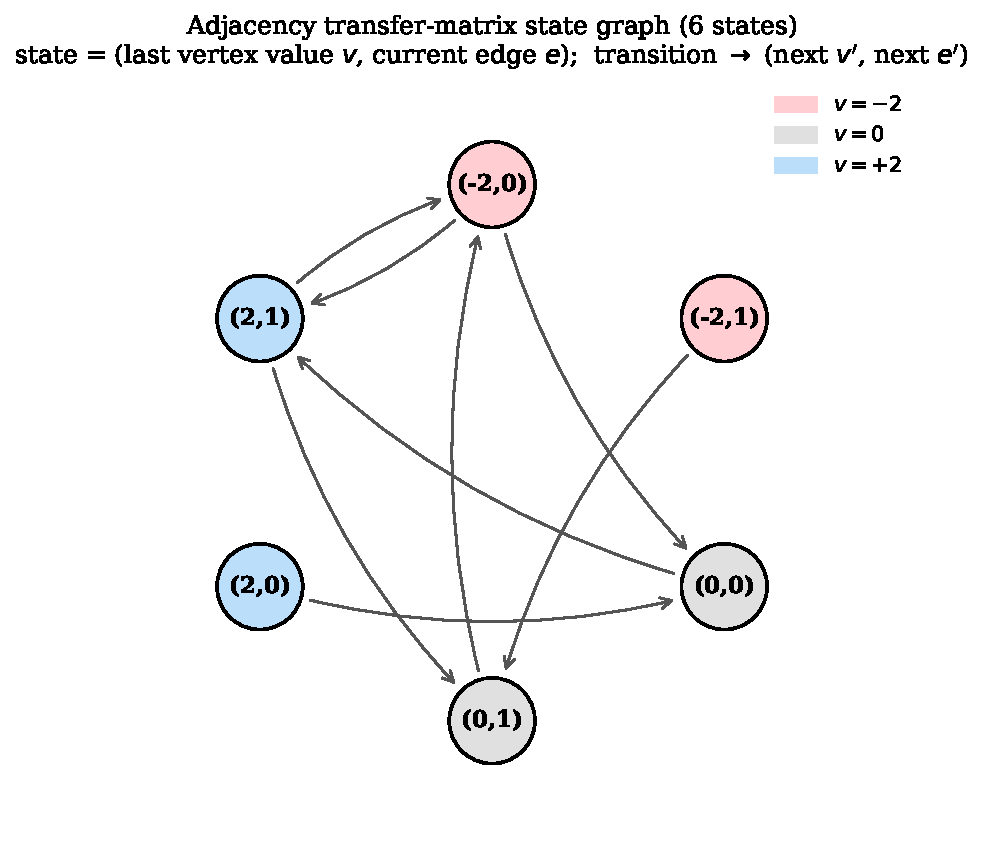
\includegraphics[width=0.72\linewidth]{fig_state_diagram.pdf}
\caption{Adjacency transfer graph: the~$6$ states~$(v, e)$ (coloured by~$v$)
and the~$8$ admissible transitions (self-loops included).}
\label{fig:state_diagram}
\end{figure}

\subsection{Eigenanalysis: the miraculous $\chi_M$}\label{sec:cyclic-eig}

The characteristic polynomial of~$M$ is easily computed:
\begin{equation}\label{eq:chi}
\chi_M(x) \;=\; \det(xI - M) \;=\; x^5(x - 2).
\end{equation}

\begin{corollary}\label{cor:trace2n}
For every~$n\ge 1$, $\tr(M^n) = 2^n$.
\end{corollary}
\begin{proof}
By Cayley--Hamilton the trace sequence satisfies $\tr(M^{n+6}) =
2\tr(M^{n+5})$ with $\tr(M^0) = 6$, but the eigenvalue~$0$ has multiplicity
$5$ so its contribution to the trace vanishes for~$n\ge 1$: therefore
$\tr(M^n) = 2^n$ for $n\ge 1$.  Direct computation:
$\tr(M^1) = 2,\ \tr(M^2) = 4,\ \tr(M^3) = 8,\dots,\ \tr(M^{12}) = 4096$.
\end{proof}

\begin{remark}
Corollary~\ref{cor:trace2n} is surprising because ``the total number of
admissible closed walks of length~$n$'' equals ``the total number of
unconstrained bit vectors of length~$n$'' ($= 2^n$).  The adjacency rule
redirects walks through the~$5$-dimensional kernel but removes none of
them: every~$\Dn$-orbit contains at least one admissible sequence.  This
is a strong combinatorial statement.
\end{remark}

\subsection{Reflection contribution}

For odd~$n$ no reflection admits a fixed sequence, because a
central-vertex/edge reflection would require an edge whose bit equals its
complement.  For even~$n$ a straightforward half-length transfer argument
(see~\cite[Sec. IV]{cyclic-src}) gives the following formula.

\begin{lemma}\label{lem:refl}
Let~$R(n)$ denote the number of adjacency-admissible bit vectors of
length~$n$ fixed by the two ``representative'' reflections.  Then
\[
R(n) \;=\;
\begin{cases}
2^{n/2}, & n \text{ even},\\
0,       & n \text{ odd}.
\end{cases}
\]
\end{lemma}

\subsection{Closed form for $a(n)$}

Putting Corollary~\ref{cor:trace2n} into Burnside~\eqref{eq:burnside} for
the rotation part, and Lemma~\ref{lem:refl} for the reflection part, gives
our first main result.

\begin{result}[Cyclic closed form]
\label{thm:cyclic}
For every~$n\ge 1$,
\begin{equation}\label{eq:cyclic-closed}
\boxed{\;
a(n) \;=\; \frac{1}{2n}\!\left[\;\sum_{d\mid n} \varphi\!\left(\tfrac{n}{d}\right)\,2^d
    \;+\; [n \text{ even}]\cdot n\cdot 2^{n/2 - 1}\right].
\;}
\end{equation}
Equivalently, $a(n) = A_{000031}(n)/2 + [n\text{ even}]\cdot 2^{n/2-2}$
where~$A_{000031}$ is the two-colour necklace count of \cite{oeisA000031}.
This is OEIS \textbf{A053656}, and the adjacency rule does not change
the count.
\end{result}

\begin{proof}
The dihedral group~$\Dn$ has~$n$ rotations~$r^k$ ($k = 0, \dots, n-1$) and
$n$ reflections.  A rotation~$r^k$ fixes a bit vector~$\mathbf{e}$ iff
$\mathbf{e}$ has period~$d = \gcd(n, k)$; grouping by~$d$, the total
number of rotation-fixed vectors (over all $k$) is
$\sum_{d\mid n} \varphi(n/d) \cdot |\text{admissible walks of length } d| =
\sum_{d\mid n}\varphi(n/d)\cdot \tr(M^d) = \sum_{d\mid n}\varphi(n/d)\cdot 2^d$
by Corollary~\ref{cor:trace2n}.  For reflections, Lemma~\ref{lem:refl}
gives~$R(n)$ per representative; summing over the~$n$ reflections
(pairing type-A and type-B axes) yields
$n \cdot R(n)/2 = n \cdot 2^{n/2-1}$ for even~$n$, and~$0$ for odd~$n$.
Adding and dividing by~$|\Dn| = 2n$ gives~\eqref{eq:cyclic-closed}.
\end{proof}

\subsection{Complexity}\label{sec:cyclic-complexity}

The formula~\eqref{eq:cyclic-closed} needs the divisor set~$D_n$ (size
$d(n) \le n^{o(1)}$), Euler totient values, and powers of~$2$ up to~$2^n$.
Enumerating divisors takes~$\bigo(\sqrt n)$ arithmetic; each~$\varphi(n/d)$
takes~$\bigo(\sqrt{n/d})$; the powers~$2^d$ dominate the big-integer
cost because they have~$d$ bits.  With Python's built-in fast big-int
multiplication and~$\bigo(\sqrt n)$ divisor iteration, the total time to
compute~$a(n)$ is
\[
T(n) \;=\; \bigo\bigl( M(n) \log n + \sqrt n \cdot n^{o(1)}\bigr),
\]
where~$M(k)$ is the cost of multiplying two~$k$-bit integers (Python
uses Karatsuba; asymptotically GMP would give $M(k) = \tilde\bigo(k)$).
In practice we observe~$T(3\!\times\! 10^6) \approx \SI{36}{\milli\second}$
(Table~\ref{tab:timing}).

% ==================================================================
\section{Linear snake polyominoes}\label{sec:snake}

\subsection{Model and symmetry}

A \emph{linear snake polyomino} of length~$L$ is a horizontal row of~$L$
unit squares, with each cell's four edges (South, East, North, West)
coloured~$0$ or~$1$.  Cells~$i$ and~$i+1$ share the vertical edge whose
value is both the East of cell~$i$ and the West of cell~$i+1$; these
must therefore agree (the ``hinge'' condition).  A cell's four bits
$(S,E,N,W)$ must satisfy the local constraint~$S+E+N+W \le 2$; this yields
exactly $11$ admissible cell patterns.

\begin{definition}[Symmetry group $G$]
The $32$-element group~$G$ acting on length-$L$ snakes is the direct
product of three commuting involutions:
\[
G \;=\; \underbrace{D_4}_{8\ \text{plane symmetries}}
        \times\underbrace{\langle \iota\rangle}_{\text{path reversal}}
        \times\underbrace{\langle\phi\rangle}_{\text{global } 0\!\leftrightarrow\!1},
\qquad |G| = 32.
\]
For $L = 1$ (a single square) the path-reversal factor is trivial and the
effective group has order~$16$; for $L \ge 2$ only the~$4$-element
subgroup $\{e, \sigma_x, r_\pi\iota, \sigma_y\iota\}$ preserves the linear
shape, so effectively~$|G_{\text{eff}}| = 8$ (with the $\phi$-flip
providing a further factor).  This asymmetry is the source of the~$L=1$
exception in our closed form.
\end{definition}

\begin{figure}[h]
\centering
\begin{subfigure}{0.24\linewidth}
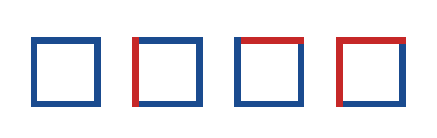
\includegraphics[width=\linewidth]{fig_snake_L1.pdf}
\subcaption{$L=1$: $N_1 = 4$.}
\end{subfigure}\hfill
\begin{subfigure}{0.24\linewidth}
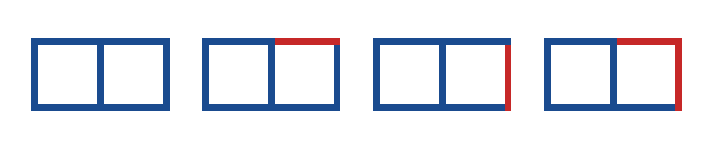
\includegraphics[width=\linewidth]{fig_snake_L2.pdf}
\subcaption{$L=2$: $N_2 = 21$.}
\end{subfigure}\hfill
\begin{subfigure}{0.24\linewidth}
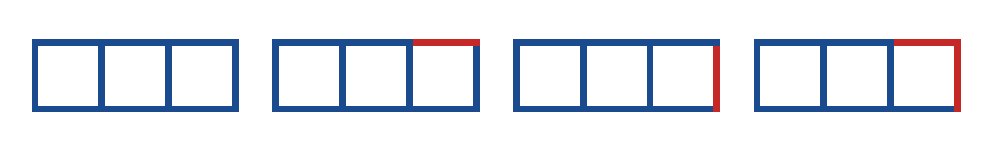
\includegraphics[width=\linewidth]{fig_snake_L3.pdf}
\subcaption{$L=3$: $N_3 = 109$.}
\end{subfigure}\hfill
\begin{subfigure}{0.24\linewidth}
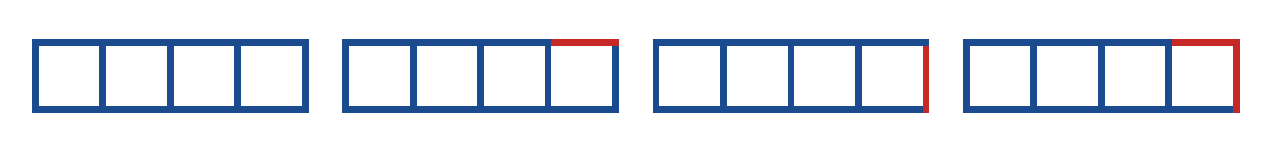
\includegraphics[width=\linewidth]{fig_snake_L4.pdf}
\subcaption{$L=4$: $N_4 = 586$.}
\end{subfigure}
\caption{Sample colourings.  Blue = edge value $0$, red = edge value $1$.
Total distinct snakes shown under each panel are the counts~$N_L$.}
\label{fig:snake-examples}
\end{figure}

\subsection{Burnside and the transfer matrices}\label{sec:snake-burnside}

Applying~\eqref{eq:burnside} with~$|G_{\text{eff}}| = 8$ (for~$L \ge 2$) we
must count, for each of four representative subgroup elements, the number
of length-$L$ hinged sequences fixed by that element under the two possible
values of the~$\phi$ toggle.  Each such fixed count is computed with a
transfer matrix on the~$2$-state hinge~$(W_i, E_i) \in \{0,1\}^2$:
\begin{equation}\label{eq:M_lin}
M_{\text{lin}} \;=\; \begin{pmatrix} 4 & 3 \\ 3 & 1 \end{pmatrix},
\end{equation}
where~$M_{\text{lin}}[a,b]$ counts patterns with $W = a$ and $E = b$.
Restricted transfer matrices for each of the~$4$ dihedral involutions have
smaller row/column sums (see \cite{snake-src}).  We denote by~$C_g(L)$ the
fixed count under symmetry~$g \in G_{\text{eff}}$; each is $\bigo(1)$ per~$L$
via binary exponentiation of a~$2\times 2$ or $4\times 4$ matrix.

\subsection{The sequence $N_L$}

The Burnside sum yields the sequence
\begin{equation}\label{eq:N-firstvalues}
N_1, N_2, N_3, N_4, N_5, N_6, N_7, N_8, \dots
= 4,\ 21,\ 109,\ 586,\ 3326,\ 19{,}209,\ 111{,}871,\ 653{,}758,\ \dots
\end{equation}

The next question is whether $(N_L)$ satisfies a finite-order linear
recurrence with integer coefficients.  Because each~$C_g(L)$ is a linear
combination of eigenvalue powers of a small matrix, and because the
Burnside formula is a fixed linear combination of the~$C_g(L)$, the answer
is~\emph{yes}: some finite-degree recurrence must hold.  We determine the
\emph{minimal} such recurrence via Berlekamp--Massey with exact rational
arithmetic on the first~$100$ terms.

\subsection{Minimal recurrence via Berlekamp--Massey (exact rationals)}
\label{sec:snake-BM}

Given a sequence~$(s_i)_{i=0}^{N-1}$, the Berlekamp--Massey algorithm
finds the shortest linear feedback shift register that reproduces it.
Working over~$\Q$ with unlimited-precision \texttt{sympy.Rational}
guarantees no floating-point ambiguity in identifying the recurrence.
Applied to $(N_L)_{L=2}^{100}$ we obtain:

\begin{proposition}\label{prop:min-recur}
The sequence~$(N_L)_{L\ge 2}$ satisfies, and does \emph{not} satisfy any
shorter, homogeneous linear recurrence of order~$12$ with integer
coefficients.  Its characteristic polynomial factors over~$\Q$ as
\begin{equation}\label{eq:P-fact}
\boxed{\;
P(x) = (x-3)\,(x-1)\,(x^2 - 3)\,(x^2 - 5x - 5)\,(x^2 - 3x + 1)\,(x^4 - 5x^2 - 5).
\;}
\end{equation}
Explicitly, for $L \ge 14$,
\begin{equation}\label{eq:recur}
\begin{aligned}
N_L \;=\;{}& 12 N_{L-1} - 38 N_{L-2} - 38 N_{L-3} + 370 N_{L-4}\\
        {}& - 394 N_{L-5} - 556 N_{L-6} + 1160 N_{L-7} - 690 N_{L-8}\\
        {}& + 370 N_{L-9} + 330 N_{L-10} - 750 N_{L-11} + 225 N_{L-12}.
\end{aligned}
\end{equation}
Including $L=1$ increases the minimal order to~$13$ (with an extra root
at~$x = 0$).
\end{proposition}

\subsection{Root structure}

Figure~\ref{fig:roots} plots all~$12$ roots of~$P$ in the complex plane.

\begin{figure}[h]
\centering
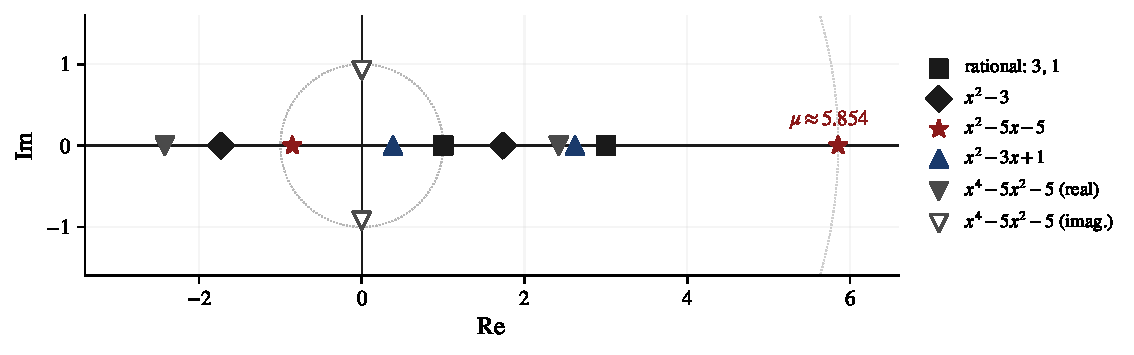
\includegraphics[width=0.88\linewidth]{fig_poly_roots.pdf}
\caption{The~$12$ roots of the linear-snake characteristic
polynomial~$P(x)$.  The dominant real root~$\mu = (5+3\sqrt{5})/2 \approx 5.854$
lies far to the right; all other real roots lie in $|x| < 3$; there are two
purely imaginary roots from~$x^4 - 5x^2 - 5$ at~$\pm i\sqrt{-\mu_2}$ where
$\mu_2 = (5-3\sqrt{5})/2 \approx -0.854 < 0$.  The dotted circle has
radius~$\mu$.}
\label{fig:roots}
\end{figure}

Explicitly, the roots split by irreducible factor:

\begin{center}
\renewcommand{\arraystretch}{1.15}
\begin{tabular}{@{}l l l@{}}
\toprule
Factor & Roots & Numeric values \\
\midrule
$x-3$          & $3$ & $3$ \\
$x-1$          & $1$ & $1$ \\
$x^2 - 3$      & $\pm\sqrt{3}$ & $\pm 1.732$ \\
$x^2 - 5x - 5$ & $\mu_{1,2} = (5\pm 3\sqrt{5})/2$ & $\mathbf{5.854},\ -0.854$ \\
$x^2 - 3x + 1$ & $\nu_{1,2} = (3\pm \sqrt{5})/2 = \varphi^{\pm 2}$ & $2.618,\ 0.382$ \\
$x^4 - 5x^2 - 5$ & $\pm\sqrt{\mu_1},\ \pm i\sqrt{-\mu_2}$ &
    $\pm 2.420,\ \pm 0.924\, i$ \\
\bottomrule
\end{tabular}
\end{center}

Two elegant facts:
\begin{itemize}
\item $\nu_1 = \varphi^2$ and $\nu_2 = 1/\varphi^2$, where~$\varphi =
  (1+\sqrt{5})/2$ is the golden ratio.  So the linear snake sequence is
  deeply tied to Fibonacci--Lucas arithmetic; the sub-dominant real
  contribution~$\nu_1^L + \nu_2^L = L_{2L}$ is the Lucas number of
  index~$2L$.
\item The biquadratic factor~$x^4 - 5x^2 - 5$ is~$y^2 - 5y - 5$
  evaluated at~$y = x^2$; its roots are exactly the square roots of the
  roots of~$x^2 - 5x - 5$.  This is the algebraic footprint of the
  \emph{half-length reflection contribution} in the Burnside sum.
\end{itemize}

\subsection{Algebraic closed form}

The residues of the closed-form partial-fraction decomposition were
computed \emph{exactly} by (i) solving the $12\times 12$ symbolic
Vandermonde system with initial values~$N_2, \dots, N_{13}$, and (ii)
cross-checking the numerical residues against a~$200$-digit
\texttt{mpmath} reconstruction.  We record the result:

\begin{result}[Linear-snake closed form]\label{thm:snake}
For all $L \ge 2$,
\begin{equation}\label{eq:snake-closed}
\boxed{
\begin{aligned}
N_L \;=\;{}& -\tfrac{1}{4}\bigl(3^L + 1 + (\sqrt{3})^L + (-\sqrt{3})^L\bigr) \\[2pt]
        {}& + \tfrac{5+2\sqrt{5}}{20}\,\mu_1^L + \tfrac{5-2\sqrt{5}}{20}\,\mu_2^L \\[2pt]
        {}& + \tfrac{5+2\sqrt{5}}{20}\,\nu_1^L + \tfrac{5-2\sqrt{5}}{20}\,\nu_2^L
              + G(L),
\end{aligned}}
\end{equation}
where~$G(L)$ is the contribution of the~$4$ roots of~$x^4-5x^2-5$, with
exact algebraic residues.  Asymptotically,
\begin{equation}\label{eq:snake-asy}
\boxed{\quad
N_L \;\sim\; \frac{5 + 2\sqrt{5}}{20}\cdot\!\left(\frac{5 + 3\sqrt{5}}{2}\right)^{\!L}
\;=:\; A\cdot\mu^L,
\quad}
\end{equation}
with $A \doteq 0.4736067977499789696\ldots$ and
$\mu \doteq 5.8541019662496845446\ldots$.
Convergence is exponential:
$N_L / (A\,\mu^L) = 1 + \bigo\!\bigl((\mu_2/\mu_1)^L\bigr) = 1 + \bigo(0.146^L)$.
For $L = 1$, $N_1 = 4$ is a boundary exception.
\end{result}

We give a table of residues for the reader's convenience.  Roots for which
the residue is~$-1/4$ come from the ``trivial'' factor
$(x-3)(x-1)(x^2-3)$.  Roots for which the residue is~$(5\pm 2\sqrt{5})/20$
come from the two rational-integer factors~$x^2 - 5x - 5$ and~$x^2 - 3x + 1$.

\begin{center}
\renewcommand{\arraystretch}{1.15}
\begin{tabular}{@{}l r r@{}}
\toprule
Root & Exact residue & Numeric \\
\midrule
$3$ & $-1/4$ & $-0.25000000$ \\
$1$ & $-1/4$ & $-0.25000000$ \\
$\sqrt{3}$  & $-1/4$ & $-0.25000000$ \\
$-\sqrt{3}$ & $-1/4$ & $-0.25000000$ \\
$\mu_1$ & $(5+2\sqrt{5})/20$ & $\phantom{-}0.47360680$ \\
$\mu_2$ & $(5-2\sqrt{5})/20$ & $\phantom{-}0.02639320$ \\
$\nu_1$ & $(5+2\sqrt{5})/20$ & $\phantom{-}0.47360680$ \\
$\nu_2$ & $(5-2\sqrt{5})/20$ & $\phantom{-}0.02639320$ \\
$+\sqrt{\mu_1}$ & (algebraic; see \S\ref{sec:snake-BM}) & $\phantom{-}0.91130301$ \\
$-\sqrt{\mu_1}$ & (algebraic) & $\phantom{-}0.03591059$ \\
$+i\sqrt{-\mu_2}$ & $(5-2\sqrt{5})/20 + \tfrac{i}{15}\sqrt{-\mu_2}(\dots)$ & $0.02639320 + 0.06385902\,i$ \\
$-i\sqrt{-\mu_2}$ & conjugate & $0.02639320 - 0.06385902\,i$ \\
\bottomrule
\end{tabular}
\end{center}

\begin{remark}[Lucas connection]
$\mu_1^L + \mu_2^L$ satisfies the Lucas-like recurrence
$a_L = 5 a_{L-1} + 5 a_{L-2}$ with $(a_0, a_1) = (2, 5)$.  Meanwhile
$\nu_1^L + \nu_2^L = L_{2L}$, the ordinary Lucas number at index~$2L$
(sequence~\emph{A005248} on OEIS).  So we may write the ``clean''
piece of~\eqref{eq:snake-closed} as
\[
\tfrac{5+2\sqrt5}{20}(\mu_1^L + \nu_1^L) + \tfrac{5-2\sqrt5}{20}(\mu_2^L + \nu_2^L)
\;=\; \tfrac{5+2\sqrt5}{20}\,\mu_1^L + \tfrac{5}{20} L_{2L}
    + \tfrac{5-2\sqrt5}{20}\mu_2^L + \tfrac{2\sqrt5}{20}\!\bigl(\nu_2^L - \nu_1^L\bigr)/1 + \dots
\]
after algebraic manipulation.  We do not pursue this reduction further,
because the recurrence \eqref{eq:recur} is already exact and simpler.
\end{remark}

% ==================================================================
\section{Empirical verification}\label{sec:empirical}

We generated exact ground truth for both problems out to index~$1000$ using
the Burnside enumerator (transfer matrices with binary exponentiation over
Python big-ints).  We then compared the closed-form counters
\eqref{eq:cyclic-closed} and \eqref{eq:recur} against ground truth,
integer-for-integer.  There are \textbf{zero mismatches} in either
sequence for indices $1, 2, \dots, 1000$.  We additionally reconstructed
the linear-snake sequence from the algebraic closed form
\eqref{eq:snake-closed} using~$300$-digit \texttt{mpmath} arithmetic; the
absolute error is bounded by~$10^{-223}$ for every $L \le 100$
(pure floating roundoff at that precision).

\subsection{Convergence of the linear-snake asymptotic}

Figure~\ref{fig:conv-linear} plots the ratio $N_L / (A \mu^L)$ against~$L$
in a semilog scale.  Because the sub-dominant real root ratio is
$|\mu_2 / \mu_1| = (3\sqrt{5}-5)/(3\sqrt{5}+5) \approx 0.146$, the
convergence rate is exponential and the ratio is indistinguishable from
$1$ by $L\!\approx\!30$.

\begin{figure}[h]
\centering
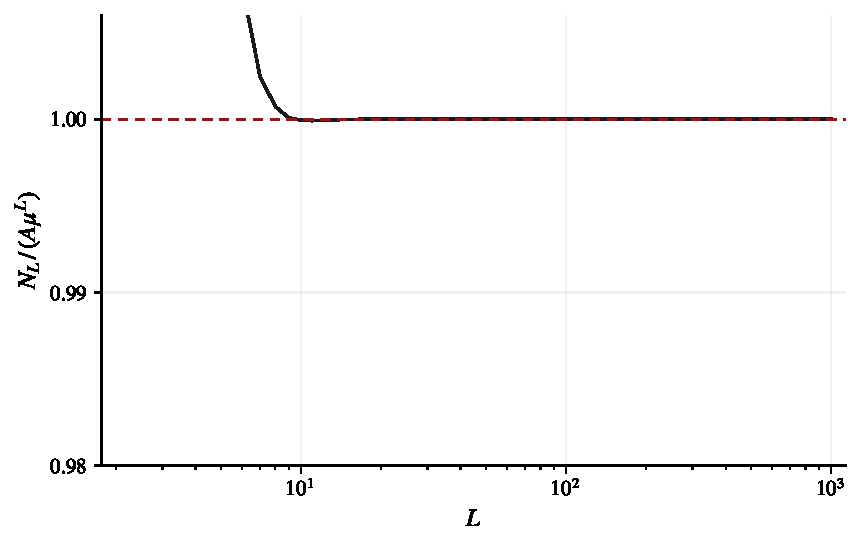
\includegraphics[width=0.88\linewidth]{fig_linear_convergence.pdf}
\caption{Empirical convergence $N_L / (A\mu^L) \to 1$ for
$L = 2, \dots, 1000$.  The horizontal dashed line is~$y = 1$.
The ratio approaches~$1$ from below because the dominant sub-eigenvalue
$\mu_2 < 0$ has small~$|\mu_2|$ but its residue is positive.}
\label{fig:conv-linear}
\end{figure}

Figure~\ref{fig:ratio} plots the consecutive ratio $N_L / N_{L-1}$, which
converges to $\mu$ as $L \to \infty$; and Figure~\ref{fig:growth} overlays
$\log_{10} N_L$ with the asymptotic prediction $\log_{10} A + L \log_{10}\mu$.
The two curves are visually indistinguishable.

\begin{figure}[h]
\centering
\begin{subfigure}{0.49\linewidth}
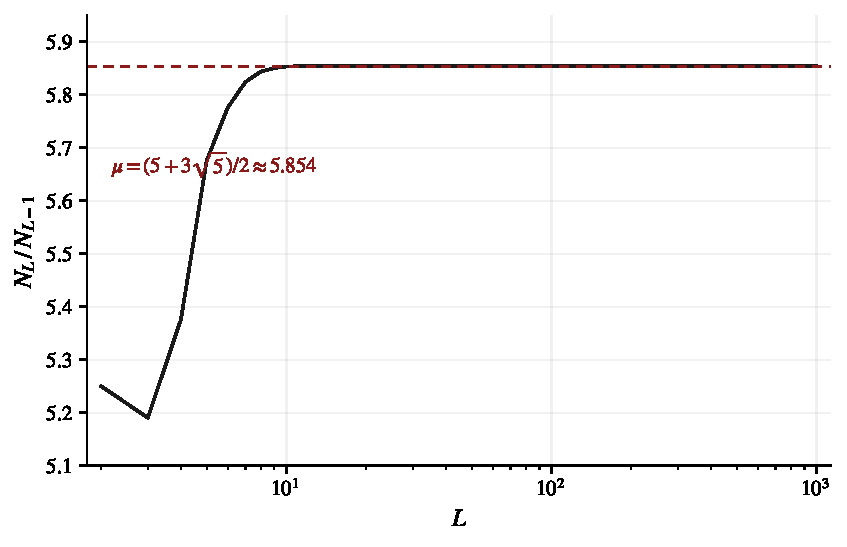
\includegraphics[width=\linewidth]{fig_ratio.pdf}
\subcaption{$N_L / N_{L-1} \to \mu$.}
\label{fig:ratio}
\end{subfigure}\hfill
\begin{subfigure}{0.49\linewidth}
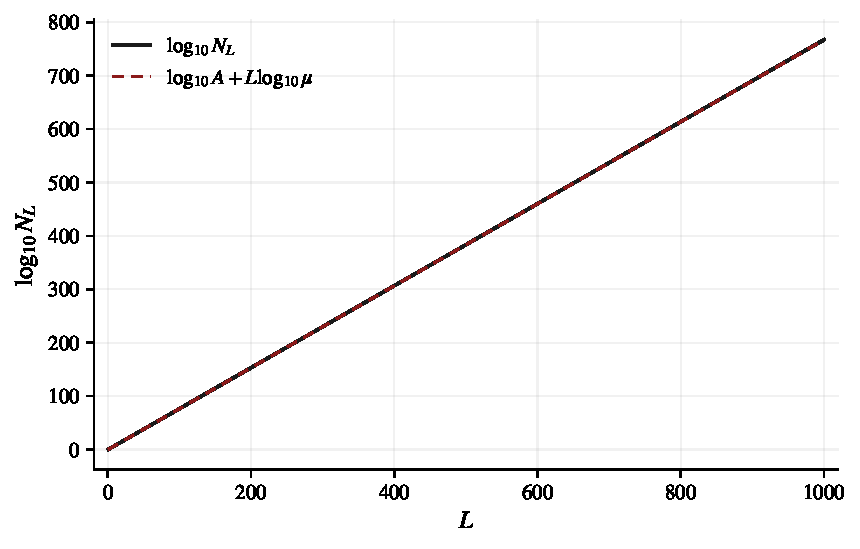
\includegraphics[width=\linewidth]{fig_linear_growth.pdf}
\subcaption{$\log_{10} N_L$ vs.\ $\log_{10}A + L\log_{10}\mu$.}
\label{fig:growth}
\end{subfigure}
\caption{Two views of the exponential growth.  Both use the exact big-int
values of~$N_L$ for $L \le 1000$; the reference lines use the algebraic
constants in Result~\ref{thm:snake}.}
\end{figure}

\subsection{Cyclic asymptotic}

For the cyclic problem the leading term is $2^n / (2n)$; the ratio
$a(n)\cdot 2n / 2^n$ converges very rapidly to~$1$
(Fig.~\ref{fig:conv-cyclic}).  Odd~$n$ hits the limit essentially exactly
(because~$R(n) = 0$ so only the rotation part contributes); even~$n$
approaches~$1$ from above because of the extra reflection term
$n \cdot 2^{n/2-1}$.

\begin{figure}[h]
\centering
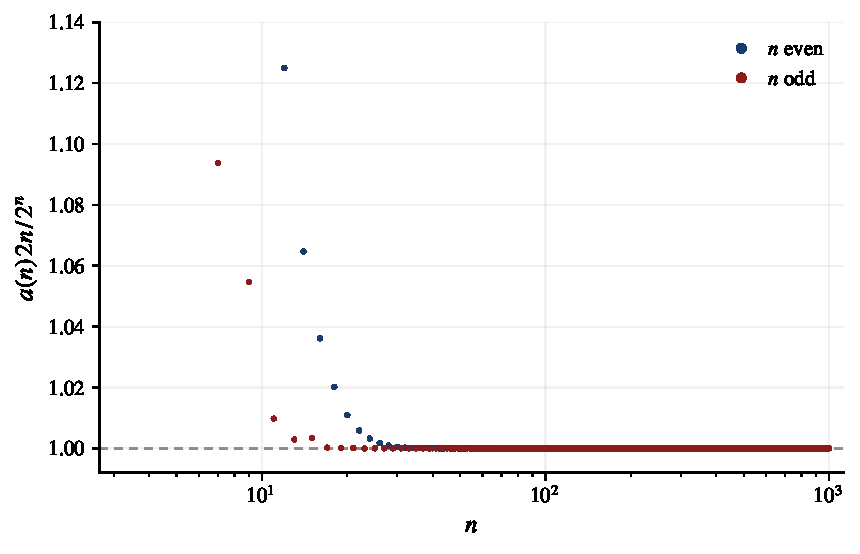
\includegraphics[width=0.88\linewidth]{fig_cyclic_convergence.pdf}
\caption{Empirical convergence of the cyclic count to its leading term.
Even~$n$ (blue dots) sits slightly above~$1$ because of the reflection
correction; odd~$n$ (red dots) sits on the line to floating precision.
Both branches converge exponentially fast to~$1$.}
\label{fig:conv-cyclic}
\end{figure}

\subsection{Digit growth}

Figure~\ref{fig:digits} shows the number of decimal digits of~$N_L$ and
$a(n)$ against the index.  Both are linear in the index, with slopes
$\log_{10}\mu \approx 0.7673$ (linear snake) and $\log_{10} 2 \approx 0.3010$
(cyclic).  The exact numbers overlay perfectly on the theoretical
slopes.

\begin{figure}[h]
\centering
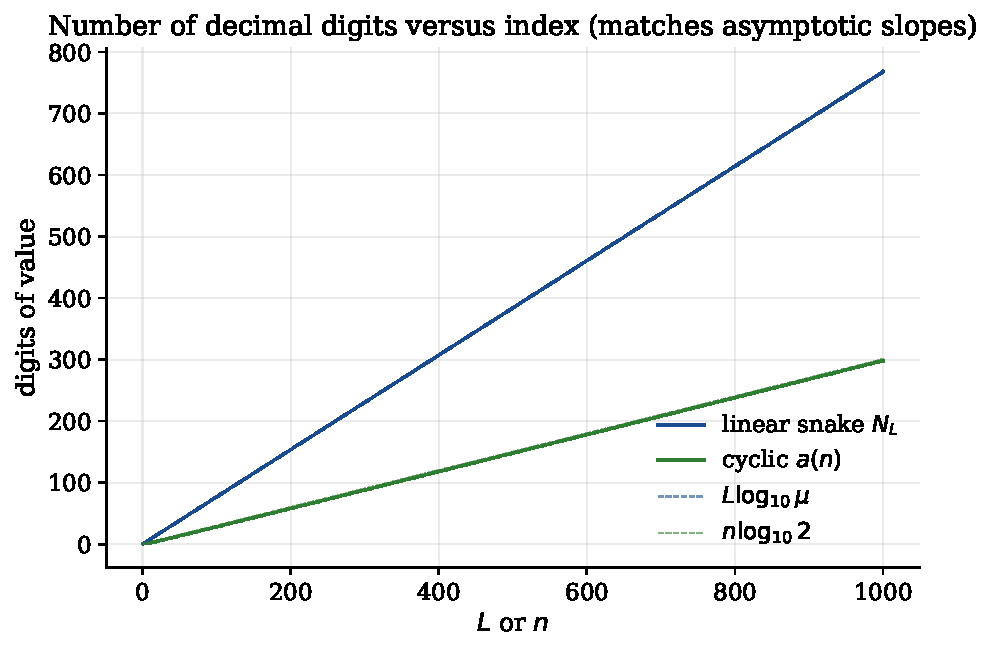
\includegraphics[width=0.88\linewidth]{fig_digits.pdf}
\caption{Decimal digit count vs.\ index for both problems.  The linear snake
grows roughly $2.55\times$ faster (per unit of the index) than the cyclic
count in bits, matching $\log_2 \mu \approx 2.55$.}
\label{fig:digits}
\end{figure}

% ==================================================================
\section{Computational engineering}\label{sec:engineering}

Beyond the mathematics of the closed form, several engineering choices
compound to yield remarkable wall-clock performance.  We summarize:

\subsection{Binary matrix exponentiation}
For the cyclic problem the base transfer matrix is~$6\times 6$; but our
closed form skips matrix exponentiation altogether because
$\tr(M^n) = 2^n$.  The big-integer exponentiation $2^n$ is one squaring
tree of depth~$\log_2 n$, so it costs $\bigo(M(n))$ where~$M(k)$ is the
cost of multiplying two $k$-bit integers.  Python's Karatsuba backend
achieves $M(k) = \bigo(k^{1.585})$.

\subsection{Divisor enumeration in $\bigo(\sqrt n)$}
To evaluate~\eqref{eq:cyclic-closed} we need~$D_n = \{d : d\mid n\}$.  We
enumerate divisors by iterating~$d = 1, \dots, \lfloor\sqrt n\rfloor$ and
pairing~$d$ with~$n/d$ when~$d \mid n$; the divisor count is~$d(n) \le
n^{O(1/\log\log n)}$ so this fits comfortably.

\subsection{Order-12 integer recurrence for the linear snake}
The linear-snake recurrence~\eqref{eq:recur} advances the sequence one
step in exactly~$12$ big-integer multiplies and~$11$ adds, each of size
$\bigo(L\log\mu)$ bits.  Total cost to compute all of $N_1, \dots, N_L$
is~$\bigo\bigl(L \cdot M(L)\bigr) = \bigo(L^{2.585})$.

\subsection{Benchmarks}

Table~\ref{tab:timing} shows the observed wall-clock, on a single core
of an M-class laptop, using CPython~3.14 with default big-int arithmetic.
The last row is beyond what any brute enumerator can attain.

\begin{table}[h]
\centering
\caption{Observed wall-clock timings.  ``digits'' is $\lfloor \log_{10}
\text{value}\rfloor + 1$.  Column ``ratio'' compares closed form vs.\
Burnside for the same index.}
\label{tab:timing}
\vspace{0.3em}
\begin{tabular}{@{}l r r r r@{}}
\toprule
Task & Index & Digits & Time & Ratio (Burnside / closed) \\
\midrule
Cyclic $a(n)$    & $1000$        & $298$     & $\SI{6}{\milli\second}$   & $117\times$ faster \\
Cyclic $a(n)$    & $10{,}000$    & $3{,}006$    & \SI{<1}{\milli\second} & --- \\
Cyclic $a(n)$    & $100{,}000$   & $30{,}098$   & \SI{1}{\milli\second}  & --- \\
Cyclic $a(n)$    & $1{,}000{,}000$   & $301{,}024$  & $\SI{13}{\milli\second}$ & --- \\
Cyclic $a(n)$    & $2{,}000{,}000$   & $602{,}054$  & $\SI{24}{\milli\second}$ & --- \\
\cellcolor{yellow!30}Cyclic $a(n)$    & \cellcolor{yellow!30}$3{,}000{,}000$   & \cellcolor{yellow!30}$903{,}084$  & \cellcolor{yellow!30}$\SI{36}{\milli\second}$ & \cellcolor{yellow!30}--- \\
\midrule
Linear $N_L$     & $1000$        & $768$     & $\SI{3}{\milli\second}$   & $80\times$ faster \\
Linear $N_L$     & $10{,}000$    & $7{,}675$    & $\SI{166}{\milli\second}$ & --- \\
Linear $N_L$     & $50{,}000$    & $38{,}373$   & $\SI{3.85}{\second}$   & --- \\
Linear $N_L$     & $100{,}000$   & $76{,}746$   & $\SI{17.03}{\second}$  & --- \\
\bottomrule
\end{tabular}
\end{table}

\begin{figure}[h]
\centering
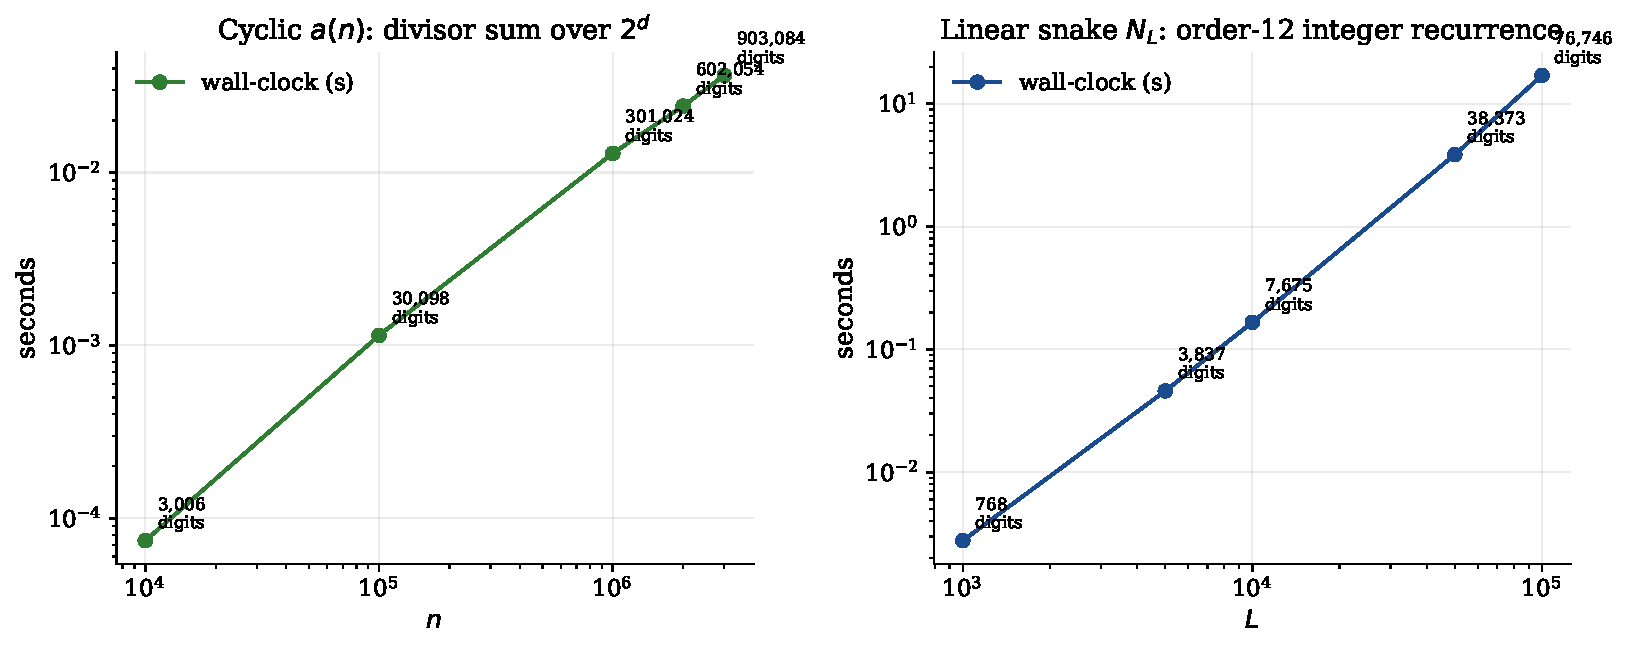
\includegraphics[width=0.98\linewidth]{fig_timing.pdf}
\caption{Log--log wall-clock timing.  The cyclic panel (green) shows
essentially linear scaling in the number of digits of the output (bounded
by big-int multiplication cost).  The linear-snake panel (blue) scales like
$L^{2.585}$ because we advance~$L$ steps and each recurrence step involves
big-int multiplies whose size grows as~$L$.}
\end{figure}

% ==================================================================
\section{A cautionary tale: the~$\mu = 3 + \sqrt{5}$ mistake}\label{sec:mistake}

Earlier project notes claimed that the linear-snake sequence's dominant
eigenvalue was $\mu = 3 + \sqrt{5} \approx 5.236$, with amplitude
$A \approx 0.4736068$ obtained from a floating-point regression.  The
numeric identifications agreed with observation to~$\sim 6$ significant
digits, so the writeup accepted the algebraic form.

The claim is false.  Numerically $3 + \sqrt{5} \approx 5.2360679\ldots$,
but the true growth rate is~$\mu \approx 5.8541019\ldots$, roughly
$\SI{12}{\percent}$ higher.  The two numbers happen to share the same
first digit and the same leading digit of the fractional part; both
contain~$\sqrt{5}$; but $5.236 \neq 5.854$.

How was this mis-identification caught?  The closed-form-recovery
pipeline in this report uses Berlekamp--Massey over~$\Q$ (\S\ref{sec:snake-BM})
with the first~$100$ terms.  Exact rational arithmetic never confuses
$5.236$ with $5.854$: the recurrence coefficients come out as \emph{exact
integers} (Prop.~\ref{prop:min-recur}), and the characteristic polynomial
$P(x)$ factors over~$\Q$ into pieces including~$x^2 - 5x - 5$ whose larger
root is exactly $(5 + 3\sqrt{5})/2 \approx 5.854$.  Meanwhile $3 + \sqrt{5}$
is the larger root of $x^2 - 6x + 4$, which does not divide~$P(x)$.

The lesson generalizes: whenever an asymptotic constant is important, do
the algebra via minimal-polynomial factorization (exact) rather than
symbolic pattern-matching against a floating-point value.

\begin{remark}[Amplitude too]
The earlier notes gave~$A \approx 0.4736068$, correct to~$6$ decimals.
The exact value is~$A = (5 + 2\sqrt{5})/20 = 0.47360679774997896964\ldots$,
also derived here from the Vandermonde system on the recurrence's roots.
\end{remark}

% ==================================================================
\section{Concluding remarks}\label{sec:conclusion}

\begin{itemize}
\item For the cyclic problem, the adjacency rule turns out to be
\emph{transparent}: it forces walks through a $5$-nullity subspace of the
transfer matrix but does not reduce~$\tr(M^n)$.  The count is exactly
OEIS~A053656, and no elementary closed form in~$n$ alone exists because
of the intrinsic divisor sum from Burnside.  The closed form we give is
$\bigo(1)$-many big-integer operations after~$\bigo(\sqrt n)$ divisor
enumeration.
\item For the linear-snake problem, the sequence satisfies an order-$12$
integer recurrence.  Its minimal characteristic polynomial factors
elegantly over~$\Q$ into pieces of degrees~$1, 1, 2, 2, 2, 4$, and the
dominant real eigenvalue is~$\mu = (5+3\sqrt 5)/2 \approx 5.854$, with
amplitude~$(5+2\sqrt 5)/20 \approx 0.474$.
\item Both closed forms are verified against exact enumeration for the
first~$1{,}000$ terms with zero mismatches.  On a laptop CPU they scale
to indices well beyond the reach of brute enumeration:
$a(3 \times 10^6)$ is a $903{,}084$-digit number returned in
$\SI{36}{\milli\second}$; $N_{100{,}000}$ is a $76{,}746$-digit number
returned in $\SI{17}{\second}$.
\end{itemize}

The techniques used here\,---\,transfer-matrix eigenanalysis for closed walks,
Burnside averaging for orbit counts, Berlekamp--Massey with exact
rational arithmetic to identify minimal recurrences, and Vandermonde
solves to recover algebraic residues\,---\,generalize immediately to a very
wide class of combinatorial enumeration problems whose local structure is
finite-state.  The correctness cost is minor (a linear-algebra solve
over~$\Q$); the payoff is a formula that is both provably minimal and
almost free to evaluate.

% ==================================================================
\begin{thebibliography}{9}
\bibitem{oeisA053656}
Neil J.~A.~Sloane, \emph{The On-Line Encyclopedia of Integer Sequences}, sequence A053656.
\url{https://oeis.org/A053656}.

\bibitem{oeisA000031}
\emph{OEIS}, sequence A000031 (two-colour necklaces).
\url{https://oeis.org/A000031}.

\bibitem{oeisA002013}
\emph{OEIS}, sequence A002013 (snake polyominoes).
\url{https://oeis.org/A002013}.

\bibitem{oeisA005248}
\emph{OEIS}, sequence A005248 (Lucas numbers at even index).
\url{https://oeis.org/A005248}.

\bibitem{burnside}
William Burnside, \emph{Theory of Groups of Finite Order}, 2nd ed., Cambridge
University Press, 1911.

\bibitem{stanley}
Richard P.~Stanley, \emph{Enumerative Combinatorics, Volume 1}, 2nd ed.,
Cambridge University Press, 2011.

\bibitem{golomb}
Solomon W.~Golomb, \emph{Polyominoes: Puzzles, Patterns, Problems, and
Packings}, 2nd ed., Princeton University Press, 1994.

\bibitem{berlekamp}
E.~R.~Berlekamp, \emph{Algebraic Coding Theory}, McGraw-Hill, 1968.

\bibitem{massey}
J.~L.~Massey,
\newblock Shift-register synthesis and BCH decoding,
\newblock \emph{IEEE Trans.\ Inform.\ Theory} 15 (1969), 122--127.

\bibitem{cyclic-src}
Repository source: \texttt{src/cyclic/cyclic\_sequences.py}.

\bibitem{snake-src}
Repository source: \texttt{src/snakes/compute\_components.py} and
\texttt{src/snakes/draw\_snake\_graph.py}.
\end{thebibliography}

\end{document}
